\documentclass[12pt,letterpaper]{article}  
%\usepackage{Rd,Sweave,upquote}  
%\usepackage{caption}  
%\usepackage{subcaption}  
\usepackage{subfig}  
\usepackage{floatpag}  
\usepackage{array}  
\usepackage{bm}
\usepackage{framed}
\usepackage[reqno]{amsmath}
\usepackage{breqn}
\usepackage{natbib,amssymb,amsthm,graphicx,verbatim,url,verbatim}  
\usepackage[all]{xy}  
\usepackage{vmargin}  
%\usepackage{comment}  
\addtolength{\hoffset}{-0.5in} \addtolength{\voffset}{-0.5in}
\addtolength{\textwidth}{0.7in} \addtolength{\textheight}{0.2in}
\usepackage{dcolumn, booktabs}  
\usepackage[dvipsnames,usenames]{color}  
\newcolumntype{.}{D{.}{.}{-1}}\newcolumntype{d}[1]{D{.}{.}{#1}}  
%\usepackage[notref]{showkeys}  
%\usepackage{endfloat}  
\usepackage{color,setspace}  

\definecolor{spot}{rgb}{0.6,0,0}  
\usepackage[pdftex, bookmarksopen=true, bookmarksnumbered=true,    
		    pdfstartview=FitH, breaklinks=true, urlbordercolor={0 1 0},    
		    citebordercolor={0 0 1}, colorlinks=true,              
		    citecolor=spot,               
		    linkcolor=spot,               
		    urlcolor=spot,              
		    pdfauthor={Soubhik Barari, Christopher Lucas, Kevin Munger},  
pdftitle={Deepfake Experiment}]{hyperref}    
% squeeze  
\usepackage{latexsym}  
\usepackage{changepage}  
% == spacing between sections and subsections  
\fontsize{12pt}{20 pt plus 1 pt minus 0.5 pt}\selectfont

\usepackage[compact]{titlesec}   
% keep floats on same page  
\renewcommand{\topfraction}{0.85}  
\renewcommand{\textfraction}{0.1}  
\renewcommand{\floatpagefraction}{0.75} % keep < \topfraction
\newcommand{\Sref}[1]{Section~\ref{#1}}  
\newcommand{\argmin}{\operatornamewithlimits{arg\,min\ }}  
\newcommand{\argmax}{\operatornamewithlimits{arg\,max\ }}  
\newcommand{\mean}{\text{mean}}    
\setstretch{1.15}
\newtheorem{claim}{Claim}
% \newcommand{\chris}[1]{\textcolor{blue}{(#1)}} % Comment this and
%                                 % uncomment the line below to remove
%                                 % my comments
% %\newcommand{\chris}[1]{} % Uncomment this to remove my comments 
\title{\bf Pre-Analysis Plan: \\ An Experiment on the Effect of Political Deepfakes on Beliefs and Attitudes\thanks{We thank the Wiedenbaum Center for generously funding this experiment. For helpful comments, we thank the Political Data Science Lab and the Junior Faculty Reading Group at Washington University in St. Louis; the Imai Research Group; the Enos Research Design Happy Hour; and American Politics Research Workshop at Harvard University. We are especially grateful to Sid Gandhi, Rashi Ranka, and the entire Deepfakeblue team for their collaboration on the production of the videos used in this project.}}  
\author{
    Soubhik Barari
    \thanks{Ph.D. Candidate, Harvard University, 
    1737 Cambridge St., Cambridge MA 02138;
    \url{soubhikbarari.org}, sbarari@g.harvard.edu}
    \and
    Christopher Lucas
    \thanks{Assistant Professor, Washington University in
      St. Louis, One Brookings Drive, St. Louis, MO 63130;
      \url{christopherlucas.org}, christopher.lucas@wustl.edu}
    \and
    Kevin Munger
    \thanks{Assistant Professor, Pennsylvania State University; \url{kevinmunger.com}, kmm7999@psu.edu}}


\date{\today}  
\begin{document}\maketitle  

\begin{abstract}
\noindent The significance of political misinformation is widely appreciated and is the focus of much ongoing research. Recent advances in machine learning present a new threat to the integrity of political information: the ability to digitally alter video footage to depict a political actor making a false or inflammatory statement with extreme realism. These synthetic videos, or ``deepfakes,'' are potentially more dangerous than existing sources of misinformation, given that video is generally treated as prima facie evidence. In this experiment, we develop a realistic, synthetic video, which we use to experimentally test whether and to what extent deepfake videos are effective at misinformation, compared to extant modes of political deception. We test a battery of heterogeneous behavioral effects on different `at-risk' subpopulations. Additionally, we test whether simply priming the existence of deepfakes -- through benign information interventions or recognition in the wild -- reduces trust in media. Finally, we provide the first descriptive evidence of the ability of a well-informed population to distinguish deepfake videos from sincere videos. In sum, these experiments serve as the first direct tests of the threat posed by previously unseen deepfake videos, along with an evaluation of our ability to ameliorate these effects through interventions that educate and prime voters.
\end{abstract}  
%TC:endignore

\clearpage

% \tableofcontents  
% \clearpage
\baselineskip=1.57\baselineskip    
\renewcommand{\baselinestretch}{1.15}

\maketitle

%% \vspace{1em}
%% \begin{center}
%% {Word Count: 11,939}
%% \end{center}
    
\section{Introduction}\label{intro}

Political misinformation is amongst the most pressing concerns in American politics. In 2019, half of the American public viewed factually inaccurate news as a bigger problem than violent crime, climate change, and terrorism \citep{mitchell2019many}. And in the 2016 presidential election, false stories about the election received more engagement than those from credible outlets \citep{silverman2016}. While misinformation's effect on the 2016 election outcome is still not well-understood, it is certain that academics, policymakers, journalists, and other stakeholders did not adequately anticipate its magnitude.

We study a new and supposedly looming threat to the integrity of political information: widespread capacity to create false videos of politicians doing and saying that which they never did nor said, colloquially termed \textit{deepfakes}. According to popular media, security experts, and even some Congressmen,  deepfakes are a near existential threat to democracy.\footnote{For example, \citet{forbes20} writes in Forbes, ``Deepfakes Are Going To Wreak Havoc On Society. We Are Not Prepared'' and \citet{galston2020} writes in Brookings, ``A well-timed forgery could tip an election.''} Testifying at an intelligence committee hearing, Senator Marco Rubio called deepfakes the ``next wave of attacks against America and western democracies'' \citep{rubio_testimony}. 

To determine the actual threat posed by deepfakes, we develop and compile a battery of novel, highly realistic deepfake videos and randomize subject exposure to these previously unseen videos. We measure different behavioral effects of exposure in comparison with existing modes of political communication of (mis)information. Finally, we benchmark the efficacy of common informational interventions thought to reduce the effects of misinformation on participant's ability to detect our novel deepfakes.

\section{Theoretical Motivation}\label{theory}

Models of electoral accountability emphasize the importance of a well-informed population of voters  \citep{barro73,holmstrom82,ferejohn86,rogoff87,fearon99,besley06}. 
Information allows voters to accurately judge candidate attributes such as leadership, expertise, competence, character, and values in order to make principled decisions at the ballot-box \citep{pierce1993political, caprara2006personality, alexander1993gender}. Misinformation, then, threatens to impair the electorate's ability to credibly evaluate their public officials \citep{hollyer2019transparency}. 

Do deepfakes pose a unique danger to an informed electorate? One view is that deepfakes are largely similar to traditional textual misinformation, for which there is an appreciable volume of research. Extant studies demonstrate that false claims that are consistent with partisan beliefs are more likely to be believed and harder to correct \citep{weeks15,nyhan2010corrections,kahan2012ideology,thorson16}. Other work documents risk factors of susceptibility such as repeated exposure \citep{pennycook2018prior}, emotional state \citep{weeks15}, age \citep{guess19}, and lazy thinking \citep{pennycook2019lazy}. However, studies largely focus on textual information and remain agnostic about these effects with regard to the medium of information delivery. Moreover, little is known about heterogeneities in behavioral effects across different subgroups. We hypothesize that video footage can more effectively manipulate two outcomes: belief in evidence and affective response towards politicians. We discuss these outcomes and their effect heterogeneities below.

\subsection{Belief in evidence}

Audiovisual media is widely considered to be \textit{prima facie} evidence. Here, we note why, and clarify how this observation underlies the expectation that deepfakes will deceive at higher rates than existing modes of misinformation. 

Most obviously, it is easier to lie with words than with video. For example, while it is trivially easy to assert that one saw aliens at Roswell, it is considerably more difficult to provide video evidence in support of this sighting. More seriously, legal precedent in the United States privileges video evidence over secondhand reporting or eyewitness testimony \citep{wallace2009watchdog}. Cellphone video recordings, public surveillance feeds, body-worn camera footage, and `hot mics' regularly capture politicians or bureaucrats engaging in violence, bribery, or other acts of wrongdoing \citep{npr2005bribes, dietrich2017bodycam, fahrenthold2016trump}. Journalists and criminal prosecutors regularly cite such footage to hold public officials legally accountable for their actions \citep{puglisi2011newspaper}. To take a recent example, during the 2016 United States presidential election, \textit{The Washington Post} published an authentic video of then-candidate Donald Trump graphically boasting of sexual misconduct. This quickly became the most viewed online article in the publication's history \citep{farhi2016trump} and was subsequently presented as evidence in later-President Donald Trump's impeachment proceedings \citep{baker2020testify}. Video-based accountability predates the Internet: footage of former president John F. Kennedy's shooting, though partially obscured and taken from a distance, was widely accepted by broadcast news anchors, criminal investigators, and the vast majority of the public as factual evidence of his assassination \citep{mchoskey1995case}\footnote{Conspiracy theories surrounding J.F.K.'s assassination dispute the identity of his shooter, not the fact of his assassination.}.

Thus, a bad-faith actor may exploit trust in video evidence in order to misinform. Given the gold standard of video-as-evidence, a sufficiently high-quality deepfake is more likely to deceive, defame, and potentially indict a political adversary than an equivalently fabricated written report of improper conduct. This motivates our first hypothesis, which is consistent with the expectations of the popular press, politicians, and policymakers regarding the effect of deepfakes.

\begin{itemize}
    \setstretch{1}
    \item[\textbf{H$_1$}:] Deepfake videos will more successfully deceive subjects that a scandal occurred compared to equivalent information conveyed via audio and text.
\end{itemize}

Existing work supports the evidentiary hypothesis. \cite{wittenberg2020minimal} finds support for the evidentiary value of video viz-a-viz the transcript of a video. They do not, however, find much evidence of additional persuasive effect of video. In Section~\ref{design}, we explore how our design breaks apart different elements of a video treatment to examine the scope conditions of this minimal result.



%TODO: do we limit the scope here to scandals or just actions/statements in general?

%KM: I like it as written. I think video works in non-scandal contexts but we aren't testing that.

\subsection{Affective appeal}

Need deepfake videos deceive -- that is, convince the viewer of a scandal that never happened -- in order to impact attitudes and beliefs? There is reason to believe not. Besides its evidentiary usage in watchdog journalism and legal testimony, video media is a powerful tool for activating emotion. The primary goal of Hollywood visual effects -- for instance, photo-realistically depicting former President John F. Kennedy shaking hands with a fictional character -- is not to persuade audiences that fictitious events actually occurred, but rather elicit affective responses through visual storytelling. Similarly, although negative campaign ads cite facts, they more successfully persuade with emotional appeals through affective language, visual frames, and musical cues \citep{brader2006campaigning}. In some cases, this response demotivates electoral participation \citep{ansolabehere1997going}. While some work questions whether negative affect manifests as unfavorable attitudes towards target candidates \citep{lau1999effects, brader2006campaigning,lau2007effects}, others discover that negative ad exposure directly decreases candidate favorability \citep{fridkin2011variability, fridkin2004negative}. 
A deepfake depicting President Barack Obama slandering a political opponent\footnote{See \url{youtube.com/watch?v=cQ54GDm1eL0}} may have a negative effect on his perceived character even if the video is not literally interpreted, much like an ad.

Additionally, political ``infotainment'' (e.g., satire, late night talk shows, comedy), the main source of political news for a large swath of Americans \citep{pew2016election}, is thought to engage audiences by cultivating both positive and negative emotional attachments to political figures and concepts \citep{baymbeyond, boukes2015odds}. Comedic impersonations that depict caricatured negative traits of politicians effectively prime viewers of those traits and can also influence viewers' electoral support \citep{esralew2012influence}.
 
In overview, if interpreted as a type of adversarial campaign message or political satire depicting a hypothetical scandal rather than documenting a real one, a deepfake may not deceive, but still solicit an affective response translating into either decreased motivation for electoral participation and/or lower politician favorability. The effects of deepfakes amongst the subgroup that is successfully deceived should be even higher. This logic motivates our next hypothesis.


\begin{itemize}
    \setstretch{1}
    \item[\textbf{H$_2$}:] Deepfake videos will have a larger effect on negative politician favorability compared to equivalent information conveyed via text and audio.
\end{itemize}

We note that we cannot disentangle the direct effect of exposure to a deepfake independent of that which operates through a mediating variable capturing whether or not a subject was deceived. While much recent work develops designs for the identification of such effects \citep{imai2011}, we leave this question to future researchers.




%\citet{wittenberg2020minimal} and \citet{vaccari2020deepfakes} study the effects of deepfakes, using a deepfake created from a widely-seen comedy sketch. These studies demonstrate [nice claim here], but are limited in the that the stimulus they use is not representative of all possible stimuli~\citep{hovland. 



%NOTES ON OUR IMPROVEMENT ON PREVIOUS STUDIES (IF NEEDED) >>>>>>>>>
% 

%, Although the magnitude of the effect size is small and limited to non-political videos. While the paper is designed to speak to the potential effects of political deepfakes, and one of their video/transcript stimuli is a deepfake video, they use \textit{exactly the same} Obama/Peele deepfake used in \cite{vaccari2020deepfakes}. 

% (CL: We don't want to seem like we're taking shots at a working paper)
% The fact that the first two (in our calculation) social science papers investigating the effects of deepfakes used the only existing example of a high-quality deepfake speaks to the difficulty of making these high-quality deepfakes. In fact, this particular video is sufficiently unique that we argue that it is not representative of how deepfakes will operate. In the Appendix, we include our correspondence with the Buzzfeed engineer who produced the deepfake. He reports using specialized equipment and combining a variety of cutting-edge video editing techniques to create the video that was then run through the deepfake algorithm. Furthermore, he ascribes much of the video's effect to the fact that Jordan Peele is a particularly talented Obama impersonator, "able to pick up on these subtle tics Jordan was doing to embody Obama."

% We argue that our novel deepfakes that are designed to approximate how deepfakes might actually be used in the context of a political campaign constitute a significant improvement in ecological validity over the existing literature.
%>>>>>>>>>>>>>>>>>>>>>>>>>>>>>>>>>>>>>>>>>>>>>>>>>>>>>>>>>>>>>>>>>>>



\subsection{Heterogeneous effects on belief and affect}

Based on a growing body of literature, we identify a number of moderator variables on the aforementioned deepfake effects. Specifically, we expect that individuals with (1) high digital literacy, (2) low political sophistication, (3) high partisan motivated reasoning, and (4) who experience prejudice confirmation are more likely to be deceived upon exposure. We believe that viewers who engage in partisan motivated reasoning and experience prejudice confirmation will also electorally penalize the target politician more. Here, we briefly define these heterogeneities and provide theoretical justification for why we might expect effects in different directions. In this section, we distinguish between \textit{causal} moderators $(^{*})$ -- that is, moderators of deepfake effects we can intervene on -- and \textit{non-causal} moderators -- that is, moderators of deepfake effects that are difficult or impossible to intervene on. Indeed, the strength of the claims between non-causal and causal moderators differ as \cite{bansak2017generalized} highlights; hence we carefully delineate the two, but interpret both types of variables as evidence of heterogeneous treatment effects.

\\[-1.5em]

% CL: this is very interesting but it doesn't seem necessary for motivating the hypothesis. Could move to appendix. 

% The effects of any media stimulus are tempered by the overall sociotechnical media environment. An influential paper \cite{bennett2008new} argued that the fractured and elective media environment at that time should entail a period of minimal effects. 

% However, developments in the past decade have changed some relevant parameters. While it remains the case that televisual media (that is, video plus audio) is the dominant modality of political content consumed by Americans, the democratization of the technology required to produce televisual media has led to an explosion of supply. Deepfakes are merely the latest iteration in a series of developments giving individuals with low-cost digital equipment the capacity to create and manipulate televisual media. Whereas twenty years ago, there were at most a few dozen hours of televisual political media created every day, today that figure is large and thus far uncounted. 

% The other significant development is the closing of the original ``digital divide" between internet users and non-users; where internet users were initially a self-selected segment of society, today fully 90\% of Americans use the internet. This has increased the importance of the ``second-level digital divide" in internet skills~\citep{hargittai2001second}. 

%TODO: need to distinguish between our intervenable digital literacy (info prompt) and the computer skills we measure in the first stage

\noindent \textbf{By digital literacy$^{*}$.} \cite{guess2020see} overview the concept of digital literacy, arguing that it is a sufficiently important moderator for online media effects now that we have exited the era of minimal effects and entered the era of heterogeneous effects. In the context of deepfakes, the logic by which we expect heterogeneous effects across levels of digital is simply that subjects with high digital literacy are more likely to distinguish deepfakes from video that was never altered. 

Much evidence suggests that digital literacy moderates misinformation effects online. %is particularly strong in the domain of ``hard" fake news in the 2016 US Presidential Election. 
For example, %Using survey data linked with Facebook data, 
\cite{guess19} report that ``users over 65 shared nearly 7 times as many articles from fake news domains as the youngest age group." during the 2016 US Presidential election. Similarly, \cite{barbera2018explaining} finds that people over 65 shared roughly 4.5 as many fake news stories on Twitter as people 18 to 24. And matching Twitter users to voter files, \cite{osmundsen2020partisan}  find that the oldest age group was 13 times more likely to share fake news than the youngest. %It remains unclear how much of these heterogeneities are due to digital literacy or to some other relevant parameter that is also correlated with age.
 
%One crucial moderator of the effect of the deepfake is whether the respondent correctly detects the video as having been manipulated, which we expect to be strongly correlated with digital literacy. Although we expect the deepfake to deceive only those subjects at the lower end of this measure, those who do interpret the video as presenting credible evidence that Elizabeth Warren said the things that are said in the video should respond very differently. 
% Because this is the central mechanism, the first dimension of our 2-stage randomization is to present half of the subjects with information about the existence of deepfakes. This should cause all subjects to be more attentive to the veracity of the video, giving us leverage on this key moderator while keeping other parameters constant. 

Applying this body of research to context of our experiment, we register the following hypothesis.

\begin{itemize}
    \setstretch{1}
    \item[\textbf{H$_{3}$}:] Deepfake videos' effect on deception will be smaller amongst subjects with high digital literacy.
\end{itemize}

\noindent \textbf{By cognition$^{*}$.} Another dimension of heterogeneity that has recently been theorized to be relevant specifically to the study of online misinformation is lazy or inattentive thinking. \cite{pennycook2019lazy} demonstrate that performance on the Cognitive Reflection Task (designed to measure the capacity to ignore initial impressions and take the time to engage higher-level thinking) is highly predictive of willingness to share fake news. %A field experiment by \cite{pennycook2019understanding}  AXX

Thus, we preregister the following hypothesis.

\begin{itemize}
    \setstretch{1}
    \item[\textbf{H$_{4}$}:] Deepfake videos' effect on deception will be smaller amongst subjects with high cognitive reflection.
\end{itemize}

\noindent \textbf{By partisan motivated reasoning.} A large literature documents how strong partisanship directs motivated reasoning about political issues even in response to new information \citep{kahan2012ideology, druckman2019evidence, bolsen2014influence, leeper2014political, enders2019informational}. Strong partisans are also more likely to be hold highly negative views of out-party elites and citizens \citep{abramowitz2018negative, iyengar2019origins,mccarty2016polarized}. As such, partisan motivated reasoning would suggest that strong partisans are more likely to believe a negative deepfake portrayal of an out-partisan politician that is consistent with with their prior negative attitudes of the target. %It is possible that lazy reasoning, not motivated reasoning is at play as in the case of headlines shared on social media \citep{pennycook2019lazy}. However, processing video information, a task demands a nominally greater degree of temporal engagement than does processing a rapid stream of short social media headlines -- in which case, 

\begin{itemize}
    \setstretch{1}
    \item[\textbf{H$_{5}$}:] Deepfake videos' effect on deception will be higher (\textbf{H$_{5a}$}) and on negative politician favorability will be higher (\textbf{H$_{5b}$}) amongst subjects with strong out-partisan identification.
\end{itemize}

\noindent \textbf{By prejudice confirmation.} Finally, much existing research demonstrates how voters' evaluation can covertly be driven by negative stereotypes, notably towards women \citep{jamieson1995beyond,teele2017ties} and racial minorities \citep{valentino2002cues,tesler2010obama}. For example, although large swathes of the American public theoretically support female politicians for office, they evaluate them according to different criteria from men \citep{bauer2020shifting}. Moreover, a sobering study finds that, next to partisanship, holding \textit{ambivalent} sexist views (rather than outright \textit{hostile} sexist views) most predicted electoral support for Trump in the 2016 election \citep{schaffner2018understanding}. One manifestation of ambivalent sexism is a descriptive norm that contemporary women violate their ``benevolent'' expectations: for instance, that women nowadays often display poor moral sensibility to men and outwardly display less aggression, offense, or anger  \citep{glick1996ambivalent}. Individuals who hold these prejudiced descriptive norms are more likely to believe a convincing fake video of a female politician that confirms their prejudice rather than disconfirms it.

%Ambivalent sexism questions have direct ties to videos:
% - Women complain about being discriminated against (--> sexist piece of shit)
% - Most women interpret innocent remarks or acts as being sexist (--> sexist piece of shit)
% - Women should remain level-headed and calm in difficult situations. (--> swearing)
% - Women should display superior moral virtue and judgment compared to men (--> shouldn't reverse position, lgbtq, etc.)
% - Women are too often uncivil, abrasive, or shrill in difficult situations. (--> )

\begin{itemize}
    \setstretch{1}
    \item[\textbf{H$_{6}$}:] Deepfake videos' effect on deception will be relatively higher amongst subjects for whom the target performs a prejudice-confirming action.
\end{itemize}

We note that there is some initial evidence that the effects of deepfakes are larger when they are combined with micro-targeting a particular audience with susceptible prior dispositions ~\citep{dobber2020microtargeted}, supporting both \textbf{H$_5$} and \textbf{H$_6$}. 

\subsection{Distrust in media}


% Although \cite{vaccari2020deepfakes} is primarily interested in \textit{cognitive} outcomes and mechanisms in contrast to our investigation of \textit{affective} ones, we agree with their investigation of the role of deepfakes in potentially increasing uncertainty and thus decreasing trust in media---or at least trust in news on social media.

The issue of uncertainty in the democratic process dates back at least to \cite{downs1957economic}, who argued that ``uncertainty arises among citizens because the costs of acquiring accurate information are too high." These costs have varied over time as information technologies have changed the way that citizens access information. One constant, as we have argued above, is that video could be treated as \textit{prima facie} evidence and thus accurate information.\footnote{This purported objectivity of images and videos was never in fact the case, as every aspect of the selection, framing and editing of these objects involved human decisions. Without resolving any debates about the \textit{correct} level of certainty in the information conveyed via videos, we maintain that the existence of deepfakes should cause a decrease in that level of certainty. } Learning about the existence of deepfakes should weaken this perception, leading to increased uncertainty in the accuracy of video information. 

Following \cite{vaccari2020deepfakes}, we expect that information about the existence of deepfakes should decrease trust. One open question is the locus of this decrease in trust. \cite{vaccari2020deepfakes} find that uncertainty prompted by deepfake exposure decrease trust ``in news on social media," but does not test for effects on ``trust in media." 

%[CL: Four paragraphs on "social media" vs "media" is a lot. I'd support trimming here, and we can extend this discussion if we get pushback.] KM: IDK I think this is conceptually tricky and we need to be clear. 

These are conceptually distinct;  in the latter,  \textit{media} refers to the central democratic institution rather than to individual ``media objects" like news broadcasts or Facebook posts. A recent review piece by \cite{schiffrin2019credibility} defines trust in media as how well people believe the media perform their role, including the tasks of selecting news and ensuring its accuracy. There is no clear analogue for ``news on social media," as no central actor is playing this role of selecting and vetting news.  
%The normative case is also different. Trust in the institution of media has been central to the practice of democracy over the past century, but has been in decline in the United States~\citep{ladd2012americans} and around the world~\citep{hanitzsch2018caught}. 
The role of social media in democracy is evolving rapidly, but trust in news on social media is currently lower than trust in other forms of media~\citep{newman2019reuters}.%, and potentially with good reason: the public and academic conversation about social media has centered on the potential issues with misinformation for years.\footnote{The prevalence of ``hard" fake news like the deceptive websites publishing fabricated stories during the 2016 appears to be limited~\citep{guess19}. However, the likelihood of encountering content of dubious provenance and veracity remains high, a problem that is endemic to the social verification of information~\citep{munger2019all}.}  

% Furthermore, there is evidence for alternative pathways between exposure to a media object and decreased trust in the institution of the media. \cite{ladd2012americans} demonstrates that experimentally providing tabloid news causes subjects report lower trust in media. Even more broadly, \cite{mutz2005new} showed that television incivility caused subjects to reduce trust in politicians, Congress and the American system of government. In contrast, \cite{munger2020null} finds that exposure to ``clickbait" headlines has no effect on ``trust in media" or ``trust in online media." 

Thus, our third hypothesis consists of an attitudinal component and behavioral component as follows:

\begin{itemize}
    \setstretch{1}
    \item[\textbf{H$_7$}:] Increasing the salience of deepfake videos will decrease trust in authentic video media (\textbf{H$_{7a}$}) and increase the false detection of deepfake videos (\textbf{H$_{7b}$}), compared to not increasing the salience of deepfake videos.
\end{itemize}


\section{Research Design}\label{design}

% Given the theoretical discussion above, our key hypotheses are as follows. First, on the logic of evidentiary persuasion, we expect that deepfakes will deceive subjects more than a comparable condition employing text. Second, on the affective appeal, we suspect that deepfakes will affect attitudes even if they do not deceive. Third, we expect exposure to deepfakes will decrease trust in media. Finally, we expect these effects to be moderated by age, digital literacy, and cognitive reflection. In this section, we explain our experimental design.

% \subsection{Sample}

We employ a survey experiment fielded to a nationally representative sample on Lucid. %Doing so permits more credible inferences about the moderating effects of age and digital literacy. 
To the extent that our sample is still not representative of the American population, we expect any bias to be downward, as the moderating effect of digital literacy is likely smaller for the subset of the population that participates in an online survey pool.

Subjects in our experiment first respond to a standard battery of demographic questions, after which they enter the first stage (\textit{exposure}) of the experiment where they are placed in a ``news feed'' -- similar to a feed found on Facebook or Twitter -- about the 2020 Democratic primary candidates, in which there may be a deepfake video. They then enter the second stage (\textit{detection}) of the experiment where they are asked to identify deepfake videos -- either before or after being debriefed about the presence of deepfake videos. In this section, we describe the experimental conditions associated with these stages. Appendix Section~\ref{sec:makingvids} describes the creation of the videos used in the \emph{exposure} stage.

% Figure X graphically illustrates the flow of the proposed experiment.

\subsection{Exposure stage}

In the first stage of our experiment, we implement a 2 x 6 factorial design, after which we measure several outcomes. %We follow this experiment with a second stage, in which all respondents are exposed to the same set of videos (some of which are doctored via deep learning and some of which are authentic depictions of a real event), and are subsequently asked to distinguish the fake from the real videos. The manipulation in this experiment is whether or not subjects are debriefed before or after this detection exercise. We now describe these manipulations, then subsequently, our experimental expectations.
The two factors in our first experiment correspond first to a randomization over treatments that we expect will moderate the evaluation of and response to media, while the second factor corresponds to exposure to one of several media (or to a control condition with no media exposure).

In the first factor, the manipulation is as follows. Subjects are assigned uniformly to either a control condition (no exposure), or a condition regarding information about the existence of misinformation and of the increased technological capacity to manipulate televisual media. This stimulus is as follows: \\

\begin{framed}
\noindent{%
    \parbox{\textwidth}{%
\textit{During the 2016 Presidential campaign, many people learned about the risk of “fake” or “zero-credibility news”: fabricated news stories posted on websites that imitated traditional news websites. While this is still a problem, there is now also the issue of digitally manipulated videos (sometimes called “deepfakes”). Tech experts are warning everyone not to automatically believe everything they read or watch online.}
}}
\end{framed}
 \\

\newline In the second factor, we randomize exposure to either a control condition (no media), a fake text condition (fake news presented only as quoted text), deepfake video (the same information as the fake text condition, but with a digitally manipulated video to corroborate the story), ``cheapfake" video (the video of the impersonator we hired to use as the base of the deepfake video) fake audio (the same audio as the deepfake and cheapfake conditions, but without the video), or to an attack ad about the subject presented in the previous deepfake videos. Each of these conditions is a media clipping of Senator Elizabeth Warren, a Democratic primary candidate at the time of writing\footnote{A key limitation of prior studies \citep{vaccari2020deepfakes} is that deepfake stimuli used are taken directly from what was (circa 2019, when the study was conducted) the highest-quality and most famous deepfake ever created: the Jordan Peele/Obama deepfake from Buzzfeed~\citep{silverman2018spot}. This both limits the external validity of such work and drastically limits the potential to re-use such stimuli in future studies as this particular video becomes highly recognizable.}.

We surround the experimentally manipulated media exposure with five media clippings, two before and three after. These reports are all real, presented either in audio, textual, or audiovisual form, and are each about a different Democratic primary candidate. The order and content of these media are fixed, and primarily serve to make mask the main manipulation in a natural ``news feed''-like environment, replicating the experience of scrolling on the Facebook News Feed. The six conditions of our manipulation are:

{ \setstretch{1}
\begin{enumerate}
    \item (\texttt{none}) No additional media about Warren.
    \item (\texttt{video}) Deepfake video and accompanying text headline of Warren (1 of following 5).
    \begin{enumerate}
        \item \textit{LEAK: Elizabeth Warren calls Joe Biden ``a piece of sh*t'' and a pedophile in call with contributor} \newline
        \item \textit{LEAK: Elizabeth Warren calls Donald Trump ``a piece of sh*t'' and a pedophile in call with contributor} \newline
        \item \textit{LEAK: Elizabeth Warren re-claims Cherokee heritage in call with contributor} \newline
        \item \textit{LEAK: Elizabeth Warren admits she doesn't ``endorse the LGBTQ lifestyle'' in call with contributor} \newline
        \item \textit{LEAK: Elizabeth Warren flips stance on student loan debt in call with contributor}
    \end{enumerate}
    \item (\texttt{audio}) Fake audio and accompanying text headline of Warren (1 of previous 5).
    \item (\texttt{text}) Fake text headline about Warren (equivalent 1 of previous 5).
    \item (\texttt{skit}) Cheapfake video (equivalent 1 of previous 5).
    \item (\texttt{ad}) Negative campaign ad video about Warren.
\end{enumerate}
}

\noindent In conditions 2-5, we randomize over multiple stories (a-e) to reduce the possibility that our results are local to a single story. The five treatment conditions are meant to simulate, though not exhaustively, different possible defamation strategies for a bad-faith actor: (a) depict incivility toward an in-party member (b) depict incivility towards an out-party member (c) prime a past controversy (d) depict a novel controversy (e) depict political insincerity. We do not register any hypotheses about heterogeneous effects across these stories within condition, but we will conduct exploratory analysis.

In the \texttt{skit} conditions, subjects are exposed to the videos used in the creation of the deepfake video, \emph{prior} to the application of the neural network. That is, this condition displays the unaltered video of the paid actress hired to impersonate Elizabeth Warren, where the exact title of the conditions 2a-e are displayed with \textit{``Leak''} replaced with \textit{``Spot-On Impersonation''}. This condition represents the most conservative test of the hypothesis that deepfake videos uniquely deceive, since it is exactly like the deepfake condition, except without the ``deepfaking," that is the computer-assisted falsification of a real politician from the actress performing the on-screen action. If we observe a difference between the \texttt{audio} and \texttt{text} conditions when compared to the deepfake condition, but not between the deepfake and the \texttt{skit} condition, it suggests that the mechanism is the video and not the falsification.

Finally, in the \texttt{ad} condition, subjects are exposed to a negative campaign ad titled, \textit{``Tell Senator Warren: No Faux Casino, Pocahontas!''}, which highlights Senator Warren's supposedly illicit support for federally funding a local casino owned by an Indian tribe, despite her previous opposition to such legislation and her false claims of Cherokee heritage. Although the ad frames Warren as politically insincere, similar to condition (e) and primes the viewer of her Cherokee heritage controversy, similar to condition (c), it stylistically and informationally differs in many other ways, and thus is not an exact ad counterfactual of our deepfake. Instead, the ad simply serves as a benchmark comparison for a deepfake's affective effect, since it is an actual campaign stimuli used in the primary election to activate negative emotions towards Warren. 

Denote a subject's particular first-stage condition as $\textsf{Exposed}_i \in \{\texttt{none},\texttt{video},\texttt{audio},\texttt{text},\texttt{skit}, \texttt{ad}\}$. After exposure to each of these manipulations, we measure our primary outcomes of interest. Specifically, we measure the three following outcomes for each subject $i$:

\begin{itemize}
    \setstretch{1}
    \item \textsf{Believe}$_i$: Whether or not the subject believes the videos they were exposed to are sincere and depicted events that actually occurred [1-5],
    \item \textsf{Favor}$_i$: General favorability toward Senator Warren as a politician [1-100],
    \item \textsf{Distrust}$_i$: To what degree the subject trusts the credibility of their media environment [1-5].
\end{itemize}

\noindent Because we do not posit any hypotheses about a respondent's item functioning on a 5-point scale (i.e. distinguishing a response of 4 vs. a response of 5), we coarsen \textsf{Believe}$_i$ and \textsf{Favor}$_i$ to binary responses. Appendix Section~\ref{sec:all_qs} notes the full survey text and all conditions, including the surrounding media, the questions measuring the outcomes denoted above, and distraction questions that we ask about the media which was not part of our experimental manipulation. Note that, following \cite{huber2007identifying} and \citep{brader2006campaigning} we measure candidate favorability using both a feeling thermometer question and a candidate vote choice question. We measure the doubt and distrust outcomes with a single question, to avoid raising suspicion about the presence of misinformation.

\subsection{Detection stage}

After completing the battery of questions in which we measure our primary outcomes of interest, the subjects begin a subsequent experimental task that measures ability to discriminate between real and fake videos. 

Before this task, half of the subjects (in addition to all of the subjects not taking part in this task) will be debriefed from the experimental condition. The other half will be debriefed after this final task. This randomization allows us to test for the effect of the debrief itself. 

Here, we employ videos created by \cite{agarwal2019protecting}, which are of lower quality (that is, detecting the video manipulation is easier) than the ones we created, in addition to using the deepfakes we created for this subsequent manipulation. We mix these videos with similar videos taken from YouTube, and expose subjects evenly to one of three conditions: no fake videos, only low-quality fake videos, mix of quality of fake videos. Appendix Section~\ref{sec:videos} displays screenshots of each of these videos.

After completing this portion of the experiment, subjects are either debriefed regarding their condition in the exposure stage or the survey immediately concludes, depending on assignment. % Section~\ref{sec:debrief} discusses this more extensively, as well as ethical considerations.

\section{Analysis}

We now lay out the exact operationalizations, specifications and associated statistical tests for each hypothesis.\footnote{For hypotheses with multiple tests, we will adjust our $p$-values via the Benjamini-Hochberg Procedure.} Unless otherwise denoted, each respondent's vector of control covariates for our outcomes of interest are given as
\begin{equation}
     \mathbf{X}_i = \Big(\textsf{Age}_i, \textsf{Race}_i, \textsf{Educ}_i, \textsf{Gender}_i,\textsf{PID}_i, \textsf{DigLit}_i, \textsf{PolKnow}_i \Big).
\end{equation}
\noindent We index theoretically relevant parameters such as the treatment effect ($\tau$) for each hypothesis test. For convenience, rather than an assertion of equality, we do not index theoretically irrelevant parameters such as each error term ($\epsilon$) or controls coefficient vector ($\beta$).

\noindent \textbf{H$_1$ (deepfake video effect on deception).} First, we test a simple difference in means belief (deception) between respondents assigned to a deepfake video vs. respondents assigned to equivalent skit or audio or text clips in the first stage. We expect that these effects will be statistically greater than 0. That is, we test the alternative hypothesis that
\begin{equation}
    \tau_{1a} = \mathbb{E} \Big[ \textsf{Believe}_i(\textsf{Exposed}_i = \texttt{video})\Big] - \mathbb{E} \Big[\textsf{Believe}_i(\textsf{Exposed}_i = \texttt{text}) \Big] > 0,
\end{equation}
and
\begin{equation}
    \tau_{1b} = \mathbb{E} \Big[ \textsf{Believe}_i(\textsf{Exposed}_i = \texttt{video})\Big] - \mathbb{E} \Big[\textsf{Believe}_i(\textsf{Exposed}_i = \texttt{audio}) \Big] > 0,
\end{equation}
and
\begin{equation}
    \tau_{1c} = \mathbb{E} \Big[ \textsf{Believe}_i(\textsf{Exposed}_i = \texttt{video})\Big] - \mathbb{E} \Big[\textsf{Believe}_i(\textsf{Exposed}_i = \texttt{skit}) \Big] > 0.
\end{equation}
% We reject the corresponding null hypothesis of $0$ average treatment via a one-tailed t-test at $\alpha$=0.05. 

\noindent Additionally, we perform a parametric test adjusting for the aforementioned control covariates via the following regression model estimated via
\begin{equation}
    \Pr(\textsf{Believe}_i=1) = \text{logit}^{-1}\Big(\bm{\tau}_1 \mathbf{1}_{\textsf{Exposed}_i}
    + \beta_{1}\mathbf{X}_i + \epsilon_i\Big),
\end{equation}

\noindent where $\mathbf{1}_{\textsf{Exposed}_i}$ is a vector of dummy variables of length 4 indicating which Warren media condition relative to \texttt{video} as the reference category that subject $i$ is assigned. %We reject the null hypothesis that the coefficients in $\bm{\tau}_1$ corresponding to the \texttt{audio} and \texttt{text} conditions are $0$ via a one-tailed t-test at $\alpha=0.05$. 

\noindent \textbf{H$_2$ (deepfake video effect on favorability).}

Equivalent to that for $H_1$, except with \textsf{Favor}$_i$ as the outcome.


\noindent \textbf{H$_3$ (heterogeneity in deception effect by digital literacy).} We conceptualize digital literacy as consisting of two components: awareness of deepfakes ($\textsf{InfoAware}_i$) specifically and experience with digital technology broadly ($\textsf{DigExp}_i$). In the context of a survey, we are able to intervene on the former, but not the latter. As such, as we test our heterogeneity hypothesis in two ways.

First, we test it using a multiplicative interactive logit model where we intervene on $\textsf{InfoAware}_i$ via an information prompt prior to the exposure stage,
\begin{equation}
    \Pr(\textsf{Believe}_i=1) = \text{logit}^{-1}\Big(\bm{\tau}_{3a}^{(1)} (\mathbf{1}_{\textsf{Exposed}_i} \times \textsf{InfoAware}_i)
    + \bm{\tau}_{3a}^{(2)}\mathbf{1}_{\textsf{Exposed}_i} + \bm{\tau}_{3a}^{(3)}\textsf{InfoAware}_i +  \beta \mathbf{X}_i + \epsilon_i\Big).
\end{equation}

\noindent We hypothesize that the marginal effect of deepfake \texttt{video} exposure (vs. \texttt{audio} or \texttt{text} or \texttt{skit} exposure) on deception will be lower when an information prompt is given. Since \texttt{video} is the reference category, this means we expect $\bm{\tau}_{4a}^{(1)}$ will be positive for the indices corresponding to and \texttt{skit}, \texttt{audio}, and \texttt{text}. %We reject the implied null hypothesis at $\alpha=0.025$, which accounts for our multiple tests.

Secondly, we test it using a multiplicative interactive linear model where the moderator is the non-intervenable $\textsf{DigExp}_i$ and the outcome is detection accuracy of deepfakes in the detection stage:
\begin{equation}
    \textsf{DetectAcc}_i = \bm{\tau}_{3b}^{(1)} (\mathbf{1}_{\textsf{Exposed}_i} \times \textsf{DigExp}_i)
    + \bm{\tau}_{3b}^{(2)}\mathbf{1}_{\textsf{Exposed}_i} + \bm{\tau}_{3b}^{(3)}\textsf{DigExp}_i +  \beta_{3b}\mathbf{X}_i + \epsilon_i
\end{equation}

\noindent We hypothesize that the marginal effect of deepfake \texttt{video} exposure (vs. \texttt{skit}, \texttt{audio}, or \texttt{text} exposure) on deception will be lower when digital literacy is higher. Since \texttt{video} is the reference category, this means we expect $\bm{\tau}_{4b}^{(1)}$ will be positive for the indices corresponding to \texttt{skit}, \texttt{audio}, and \texttt{text}. % We reject the implied null hypothesis at $\alpha=0.025$, which accounts for our multiple tests.

% The specification for testing this hypothesis is given as a multiplicative interaction linear model:
%\begin{equation}
%    \textsf{DetectAcc}_i = \bm{\tau}_{5}^{1} (\mathbf{1}_{\textsf{Exposed}_i} \times \textsf{InfoAcc}_i)
%    + \bm{\tau}_{5}^{2}\mathbf{1}_{\textsf{Exposed}_i} + \bm{\tau}_{5}^{3}\textsf{CR}_i + \mathbf{1}_{\textsf{Exposed}_i} \beta_{5}\mathbf{X}_i + \epsilon_i
%\end{equation}

%where $\mathbf{X}_i$ is the same as before but not does not include $\textsf{CR}_i$. $\bm{\tau}_{5}^{1}$ is the moderating effect of cognitive reflection on deepfake deception, which we hypothesize to be negative. 



%Since we intervene on cognitive reflection via an accuracy prompt, we ...

%TODO: is the accuracy prompt an intervention on cognitive reflection? are they separate? 
%      presumably we care about both's effect on accuracy, but not sure how to specify this exactly %%KM I'm taking this from Pennycook/Rand/Eckle's paper:

% I think the framework above works perfectly here

\noindent \textbf{H$_4$ (heterogeneity in deception effect by cognition).} We conceptualize cognition as consisting of two components: the salience of accuracy ($\textsf{InfoAcc}_i$)  and the subject's trait level of cognitive reflection ($\textsf{CR}_i$). In the context of a survey, we are able to intervene on the former, but not the latter. As such, as we test our heterogeneity hypothesis in two ways.

First, we test it using a multiplicative interactive logit model where we intervene on $\textsf{InfoAcc}_i$ via an accuracy prompt prior to the exposure stage,
\begin{equation}
    \Pr(\textsf{Believe}_i=1) = \text{logit}^{-1}\Big(\bm{\tau}_{4a}^{(1)} (\mathbf{1}_{\textsf{Exposed}_i} \times \textsf{InfoAcc}_i)
    + \bm{\tau}_{4a}^{(2)}\mathbf{1}_{\textsf{Exposed}_i} + \bm{\tau}_{4a}^{(3)}\textsf{InfoAcc}_i +  \beta \mathbf{X}_i + \epsilon_i \Big).
\end{equation}

\noindent We hypothesize that the marginal effect of deepfake \texttt{video} exposure (vs. \texttt{skit}, \texttt{audio}, or \texttt{text} exposure) on deception will be lower when an information prompt is given. Since \texttt{video} is the reference category, this means we expect $\bm{\tau}_{4a}^{(1)}$ will be positive for the indices corresponding to \texttt{skit}, \texttt{audio}, and \texttt{text}. % We reject the implied null hypothesis at $\alpha=0.025$, which accounts for our multiple tests.

Secondly, we test it using a multiplicative interactive linear model where the moderator is the non-intervenable $\textsf{CR}_i$ and the outcome is detection accuracy of deepfakes in the detection stage:
\begin{equation}
    \textsf{DetectAcc}_i = \bm{\tau}_{4b}^{(1)} (\mathbf{1}_{\textsf{Exposed}_i} \times \textsf{CR}_i)
    + \bm{\tau}_{4b}^{(2)}\mathbf{1}_{\textsf{Exposed}_i} + \bm{\tau}_{4b}^{(3)}\textsf{CR}_i +  \beta_{4b}\mathbf{X}_i + \epsilon_i
\end{equation}

\noindent We hypothesize that the marginal effect of deepfake \texttt{video} exposure (vs. \texttt{skit}, \texttt{audio}, or \texttt{text} exposure)  on deception will be lower when digital literacy is higher. Since \texttt{video} is the reference category, this means we expect $\bm{\tau}_{4b}^{(1)}$ will be positive for the indices corresponding to \texttt{skit}, \texttt{audio}, and \texttt{text}. % We reject the implied null hypothesis at $\alpha=0.025$, which accounts for our multiple tests.

\noindent \textbf{H$_{5a}$ (heterogeneity in deception effect by partisanship).} The specification for testing this hypothesis is given as a multiplicative interaction binary regression:
\begin{equation}
    \Pr(\textsf{Believe}_i=1) = \bm{\tau}_{5a}^{(1)} (\mathbf{1}_{\textsf{Exposed}_i} \times \textsf{PID}_i)
    + \bm{\tau}_{5a}^{(2)}\mathbf{1}_{\textsf{Exposed}_i} + \bm{\tau}_{5a}^{(3)}\textsf{PID}_i +  \beta_{5a}\mathbf{X}_i + \epsilon_i
\end{equation}

\noindent where $\mathbf{X}_i$ is the same as before but not does not include $\textsf{PID}_i$. $\bm{\tau}_{6}^{(1)}$ is the moderating effect of Republican partisanship on deepfake deception, which we hypothesize to be positive. Note that $\bm{\tau}_{6}^{(1)}$ cannot be interpreted as a causal moderator. 

\noindent \textbf{H$_{5b}$ (heterogeneity in favorability effect by partisanship)}

As above, except with \textsf{Favor}$_i$ as the outcome.

\noindent \textbf{H$_{6}$ (heterogeneity in deception effect by prejudice confirmation)}

As in H$_{5a}$, except substituting prejudice confirmation in the interaction.

%TODO: should be straight-forward once we figure out the above

\noindent \textbf{H$_{7a}$ (deepfake salience effect on media distrust).} After the first stage exposure, we query our respondents about their level of trust in the media. Prior to measuring this outcome, in the context of our experiment, we argue that the idea of deepfakes can be made salient in three ways:
\begin{enumerate}
    \setstretch{1}
    \item[(I)] By receiving an information prompt about deepfakes before the first stage,  $\textsf{InfoAware}_i = 1$.
    \item[(II)] By recognizing that the stimulus is a deepfake in the first stage,  $\mathbf{1}\{\textsf{Exposed}_i = \texttt{video} \} \times \textsf{Belief}_i = 1$.
\end{enumerate}
In (I) and (II), we expect this increased salience to increase the likelihood of the respondent reporting distrust in the media. As such, we perform the corresponding two tests:
\begin{align}
    \Pr(\textsf{Distrust}_i = 1) & = \text{logit}^{-1}\Big(\bm{\tau}_{7a_{\text{I}}} \textsf{InfoAware}_i 
    + \beta \mathbf{X}_i + \epsilon_i\Big) \\
    \Pr(\textsf{Distrust}_i = 1) & = \text{logit}^{-1}\Big(\bm{\tau}_{7a_{\text{II}}} (\mathbf{1}\{\textsf{Exposed}_i = \texttt{video} \} \times \textsf{Belief}_i)
    + \beta_{7a_{\text{II}}}\mathbf{X}_i + \epsilon_i\Big)
\end{align}

\noindent \textbf{H$_{7b}$ (deepfake salience effect on false detection).} We expect that increased salience of deepfakes will increase the false detection rate of deepfakes in the detection stage of our experiment. In addition to the ways stipulated above in \textbf{H$_{7a}$} that deepfakes can be primed before the \textit{exposure} stage, there are two additional ways deepfakes can be primed ahead of the \textit{detection} stage:

\begin{enumerate}
    \setstretch{1}
    \item[(III)] By being debriefed that the stimulus in the first stage was a deepfake before entering the second stage rather than at the end of the experiment, $\mathbf{1}\{\textsf{Exposed}_i = \texttt{video} \} \times \textsf{DebriefBefore}_i = 1$.
    \item[(IV)] By receiving an accuracy prompt directing the respondent's attention on fake news content, $\textsf{InfoAcc}_i = 1$.
\end{enumerate}

\noindent Taken together, these different ways of raising salience of deepfakes imply a series of multiplicative linear models:
\begin{align}
    \textsf{DetectAcc}_i & = \tau_{7b_{\text{I}}} \textsf{InfoAware}_i + \beta \mathbf{X}_i + \epsilon_i \\
    \textsf{DetectAcc}_i & = \tau_{7b_{\text{II}}} (\mathbf{1}\{\textsf{Exposed}_i = \texttt{video} \} \times \textsf{Belief}_i) + \beta \mathbf{X}_i + \epsilon_i \\
    \textsf{DetectAcc}_i & = \tau_{7b_{\text{III}}} (\mathbf{1}\{\textsf{Exposed}_i = \texttt{video} \} \times \textsf{DebriefBefore}_i) + \beta \mathbf{X}_i + \epsilon_i \\
    \textsf{DetectAcc}_i & = \tau_{3b_{\text{IV}}}\textsf{InfoAcc}_i  + \beta \mathbf{X}_i + \epsilon_i
\end{align}

%TOOD: distinguish between causal vs. non-causal


\section{Ethics}\label{sec:debrief}


We highlight the ethical considerations pursuant to a study that uses stimuli which we expect to be uniquely deceptive. 

First, in addition to the subjects randomly assigned to a debrief in the middle of the survey, we extensively debrief all subjects at the completion of the survey (see Section~\ref{sec:all_qs} for the full text of the debriefing). This debrief goes beyond the standard description of study procedures. We require respondents to type out the following phrase, depending on which experimental arm they were assigned to:
\begin{framed}
\noindent{%
    \parbox{\textwidth}{%
\textit{``The [video/audio/text] about Elizabeth Warren is false."}
}}
\end{framed}

Second, to minimize the risk of influencing the proximate election, we opted to make a deepfake of high-profile 2020 Democratic Presidential candidate who was not ultimately selected as the nominee. Elizabeth Warren is a salient politician, making our experiment more ecologically valid than one with a low-profile or hypothetical politician, but she is slated for re-election until 2024. We selected a female candidate because women are more likely to be the targets of non-political deepfakes, and we specifically test for whether pre-existing prejudice against women among subjects changes the effect of the deepfake. Two of the treatments do refer to Presidential nominees Trump and Biden, but since they are otherwise identical, any effects they produce would be offset.

Third, we carefully weigh the risks to subjects against the potential risks that may be averted with the knowledge gained through our experiment. The potential long-term consequences of exposure to a single piece of media are minimal. That is, participants are unlikely to change their political behavior as a response to treatment, given our extensive debrief. Given that we have no experimental evidence either way, it is at least as likely that our experiment will \textit{benefit} subjects as cause harm. The experiment gives subjects experience detecting fake media, followed up by the debrief which contains feedback and information about how the deepfake process works. Given the importance and seeming inevitability of more deepfakes in the future, and the uncertainty around their effects, we argue that academics in fact have an ``obligation to experiment"~\citep{ko2016obligation}. We believe that improved understanding of how deepfakes function and evidence from our low-cost interventions will in fact serve to prevent real-world harms from deepfakes in the future.


Finally, a similar argument applies to the knowledge we generate from the perspective of policy-makers, journalists, and election administrators \citep{agarwal2019protecting}. More specifically, our study can inform future legislation or platform policies designed to minize the threat posed by this technology.\footnote{See \texttt{SB 6513} introduced in the \href{https://apps.leg.wa.gov/billsummary/?BillNumber=6513&Year=2020&Initiative=false}{WA state legislature} at the time of writing, intended to restrict the use of deepfake audio or visual media in campaigns for elective office.}


\singlespace  
\bibliographystyle{apsr}   
%\bibsep=0in   
\bibsep=\baselineskip  
\pdfbookmark[1]{References}{References}  
\bibliography{deepfake_refs}  
\setstretch{1.5}
\appendix

\section{Complete Survey}\label{sec:all_qs}

\section{Developing deepfakes}\label{sec:makingvids}

Deepfakes that swap the face of a \textsf{target} (e.g., President Barack Obama) with an \textsf{actor} (e.g., Hollywood actor Jordan Peele) are synthesized via a particular class of artificial neural networks called Adversarial Autoencoders \citep{makhzani2015adversarial}. 

The deepfaker's task is to train two autoencoders to accurately represent (encode) the two respective faces in a latent space and accurately reconstruct (decode) them as images. Let $\mathbf{X}_{\textsf{target}}$ denote a set of facial images of the target and $\mathbf{X}_{\textsf{actor}}$ denote a set of facial images of the actor. Denoting $\mathcal{G}_{\textsf{target}}$ as the function for the target autoencoder and $\mathcal{G}_{\textsf{actor}}$ as the function for the actor autoencoder, the networks are structured as $\mathcal{G}_{\textsf{target}}(x) = \delta_{\textsf{target}} \big\{\pi(x) \big\}$ and $\mathcal{G}_{\textsf{actor}}(x^\prime) = \delta_{\textsf{actor}} \big\{\pi(x^\prime) \big\}$ where $\pi$ is an encoder subnetwork, $\delta_{\textsf{target}}$ and $\delta_{\textsf{actor}}$ are the decoder subnetworks for the target and actor respectively, and $x \in \mathbf{X}_{\textsf{target}}, x^\prime \in \mathbf{X}_{\textsf{actor}}$. Both autoencoders share an encoder function $\pi$ which discover a common latent representation for the targets' and actors' faces; separate decoders are charged with realistically reconstructing the input faces. The objective function to be optimized is:

\begin{equation}\label{adversarial}
\min_{ \substack{\pi, \\ \delta_{\textsf{target}}, \\ \delta_{\textsf{actor}} } } \mathbb{E}_{x \sim \mathbf{X}_{\textsf{target}} }\Big[ || \delta_{\textsf{target}} \big\{\pi(x) \big\} - x ||^2 \Big] + \mathbb{E}_{x^\prime \sim \mathbf{X}_{\textsf{actor}} }\Big[ || \delta_{\textsf{actor}} \big\{\pi(x^\prime) \big\} - x^\prime ||^2 \Big]
\end{equation}

\noindent To produce a deepfake given a audiovisual performance of the actor with respective facial image frames $\mathbf{Y}_{\textsf{actor}} = \Big[y_1, \ldots, y_N \Big]$, we input the frames into the trained target autoencoder which outputs $\mathbf{Y}_{\textsf{actor}} = \Big[\delta_{\textsf{target}}\big\{\pi(y_1)\}, \ldots, \delta_{\textsf{target}}\big\{\pi(y_N)\}\Big]$ that can be recombined with the audio of the actor's performance.

To maximize the realism of outputs created from actor inputs fed to the target autoencoder, we train a third discriminator neural network $\mathcal{D}$ which aims to accurately classify the latent representations of images as belonging to either the target or actor. The final adversial objective is given as:

\begin{equation}\label{adversarial_loss}
\setstretch{1}
\begin{gathered}
\max_{\mathcal{D}} \min_{ \substack{\pi, \\ \delta_{\textsf{target}}, \\ \delta_{\textsf{actor}} } } \mathbb{E}_{x \sim \mathbf{X}_{\textsf{target}} }\Big[ || \delta_{\textsf{target}} \big\{\pi(x) \big\} - x ||^2 \Big] + \mathbb{E}_{x^\prime \sim \mathbf{X}_{\textsf{actor}} }\Big[ || \delta_{\textsf{actor}} \big\{\pi(x^\prime) \big\} - x^\prime ||^2 \Big] \\ + \quad \mathbb{E}_{x^{\prime\prime} \sim \mathbf{X} }\Big[ ||\mathcal{D}\big\{ \pi(x^{\prime\prime})\big\} - \mathbf{1}\{ x^{\prime\prime} \in \mathbf{X}_{\textsf{actor}} \}||^2 \Big]
\end{gathered}
\end{equation}

\noindent Optimization of this objective function can be performed via alternating iterative updating of the two networks' weights using stochastic gradient descent. After sufficient rounds of training, the target autoencoder can accurately reproduce the target's face using images of only the actor's face and is thus able to effectively `fool' the discriminator. Figure~\ref{fig:pipeline} graphically illustrates the resulting  procedure for producing deepfake face-swap videos.

\begin{figure}[h]
    \centering
    %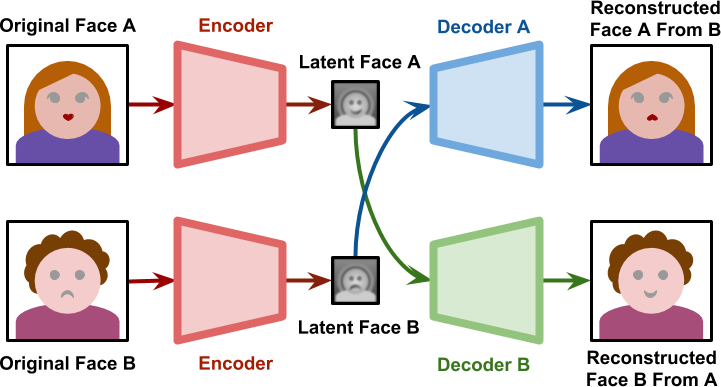
\includegraphics[width=0.8\textwidth]{deepfake_test.png}
    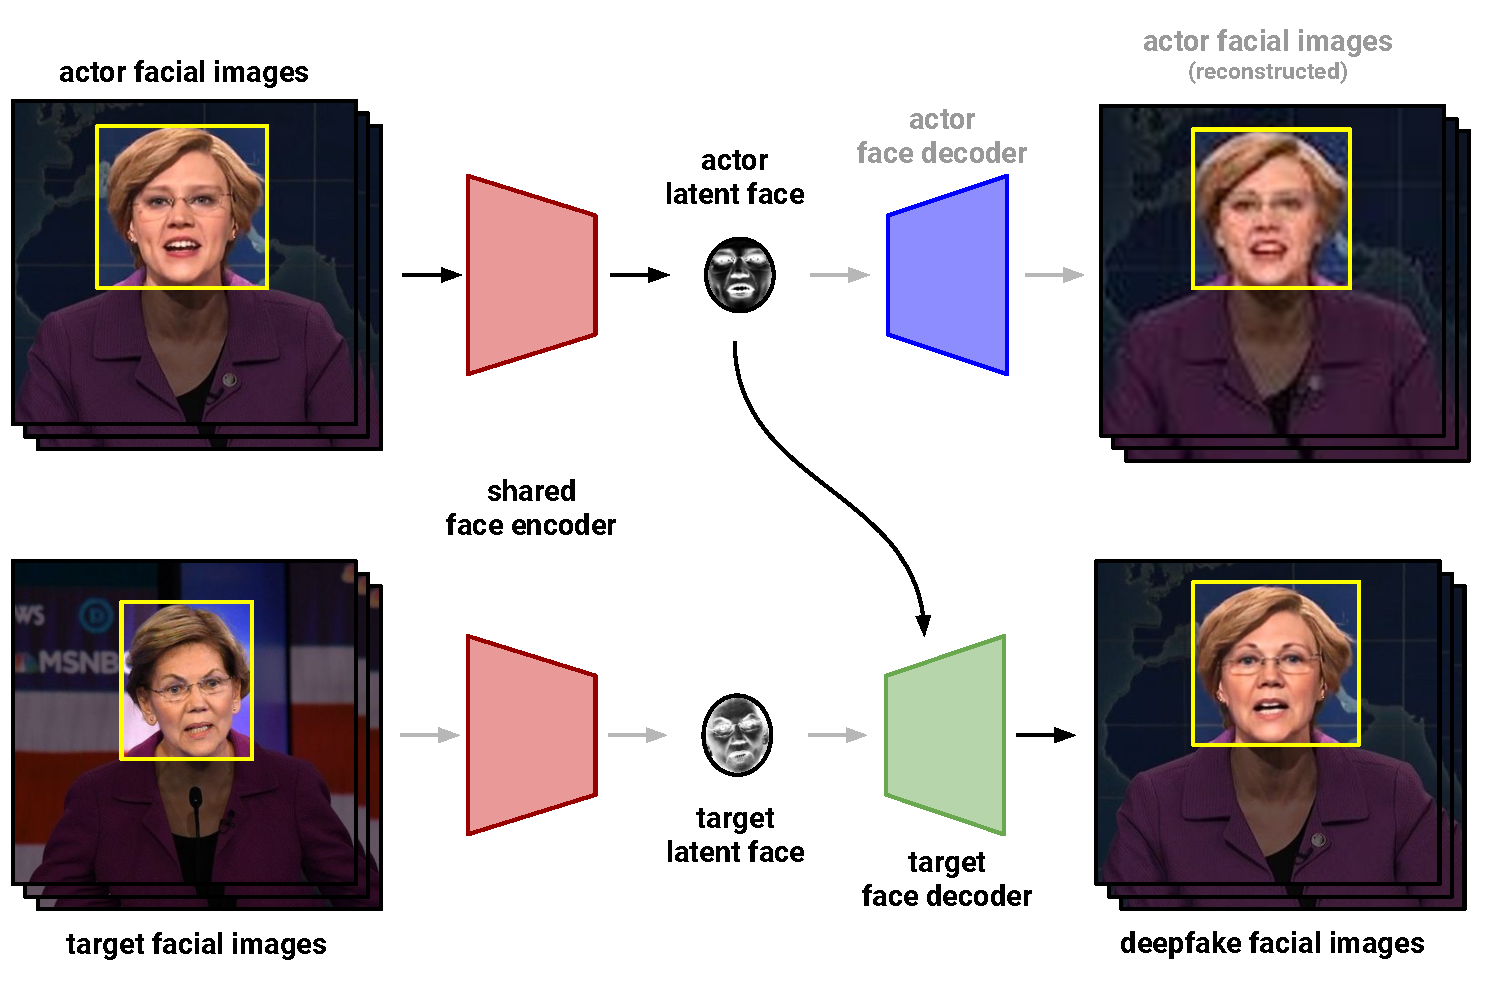
\includegraphics[width=\textwidth]{faceswap_illustration.pdf}
    \setstretch{1}
    \caption{\textbf{Deepfake Image Frame Generation via Face-swap.} This graphic illustrates the process of generating the individual image frames of a deepfake video via face-swap. First, an autoencoder network $\mathcal{G}_{\textsf{actor}}$ is trained to accurately represent/encode and reconstruct/decode facial images of an actor (top) and a network $\mathcal{G}_{\textsf{target}}$ is trained to do the same for a target (bottom). Then, to execute the face-swap, the latent representation of each frame of the actor's performance are decoded using the target network's decoder (green), rather than the actor network's decoder (blue). Shown in the lower right are the resulting ``deepfake'' facial images (yellow box) seamlessly edited back onto the actor's background. Finally, the deepfake images are combined with the actor's original vocal performance to create the deepfake video. }
    \label{fig:pipeline}
\end{figure}

In practice, this workflow for deepfake synthesis is implemented using the \texttt{TensorFlow} library \citep{abadi2016tensorflow}. Deepfake producers utilize code from several popular public code repositories which implement variants of this base framework -- including multiple discriminators and autoencoders, regularization schemes, and particular network architecture choices.

In collaboration with an industry partner\footnote{See \url{https://dfblue.com/}}, we produced a series of deepfake videos using target footage of 2020 presidential candidate Elizabeth Warren and actor performances of a professional Elizabeth Warren impersonator. We describe the content of the performances which are used in the first stage of our experiment in the next section.

\section{Video Treatments}\label{sec:videos}

\subsection{Real Videos}

\subsection{Fake Videos}

%% \color{red}
%% \section{TODO: OLD TEXT}
%% \input{old_text_to_merge} 

\end{document}
